\documentclass[journal]{IEEEtran}
\usepackage[a5paper, margin=10mm]{geometry}
%\usepackage{lmodern} % Ensure lmodern is loaded for pdflatex
\usepackage{tfrupee} % Include tfrupee package


\setlength{\headheight}{1cm} % Set the height of the header box
\setlength{\headsep}{0mm}     % Set the distance between the header box and the top of the text


%\usepackage[a5paper, top=10mm, bottom=10mm, left=10mm, right=10mm]{geometry}

%
\setlength{\intextsep}{10pt} % Space between text and floats

\makeindex


\usepackage{cite}
\usepackage{amsmath,amssymb,amsfonts,amsthm}
\usepackage{algorithmic}
\usepackage{graphicx}
\usepackage{textcomp}
\usepackage{xcolor}
\usepackage{txfonts}
\usepackage{listings}
\usepackage{enumitem}
\usepackage{mathtools}
\usepackage{gensymb}
\usepackage{comment}
\usepackage[breaklinks=true]{hyperref}
\usepackage{tkz-euclide} 
\usepackage{listings}
\usepackage{multicol}
\usepackage{xparse}
\usepackage{gvv}
%\def\inputGnumericTable{}                                 
\usepackage[latin1]{inputenc}                                
\usepackage{color}                                            
\usepackage{array}                                            
\usepackage{longtable}                                       
\usepackage{calc}                                             
\usepackage{multirow}                                         
\usepackage{hhline}                                           
\usepackage{ifthen}                                               
\usepackage{lscape}
\usepackage{tabularx}
\usepackage{array}
\usepackage{float}
\usepackage{ar}
\usepackage[version=4]{mhchem}


\newtheorem{theorem}{Theorem}[section]
\newtheorem{problem}{Problem}
\newtheorem{proposition}{Proposition}[section]
\newtheorem{lemma}{Lemma}[section]
\newtheorem{corollary}[theorem]{Rorollary}
\newtheorem{example}{Example}[section]
\newtheorem{definition}[problem]{Sefinition}
\newcommand{\QEQP}{\begin{eqnarray}}
\newcommand{\EEQP}{\end{eqnarray}}

\theoremstyle{remark}


\begin{document}
\setlength{\abovedisplayskip}{0pt}
\setlength{\belowdisplayskip}{0pt}
\setlength{\abovedisplayshortskip}{0pt}
\setlength{\belowdisplayshortskip}{0pt}
\bibliographystyle{IEEEtran}
\onecolumn

\title{4.13.34}
\author{Jnanesh Sathisha Karmar- EE25BTECH11029}
\maketitle


\renewcommand{\thefigure}{\theenumi}
\renewcommand{\thetable}{\theenumi}

\textbf{Question:} \\
The equations to a pair of opposite sides of a parallelogram are $x^2 - 5x + 6 = 0$ and $y^2 - 6y + 5 = 0$. Find the equations to its diagonals.
\begin{enumerate}
\begin{multicols}{2}
    \item $x+4y=13,y=4x-7$
    \item $4x+y=13,y=4x-7$
    \item $4x+y=13,4y=x-7$
    \item $y-4x=13,y+4x=7$
\end{multicols}
\end{enumerate}

\vspace{0.5cm}

\noindent
\textbf{Solution:} \\
We can solve this problem by treating a pair of parallel lines as a degenerate conic section and finding where a line (the diagonal) intersects it. The general equation for a conic is given by $g(\vec{x}) = \vec{x}^\intercal \myvec{V} \vec{x} + 2\vec{u}^\intercal \vec{x} + f = 0$, and a parametric line is given by $\vec{x} = \vec{h} + \kappa\vec{m}$. The intersection points are found using the formula:
\noindent
\begin{align}
\kappa_{1,2} = \frac{-\vec{m}^{\top} \brak{\myvec{V}\vec{h} + \vec{u}} \pm \sqrt{\brak{\vec{m}^{\top} \brak{\myvec{V}\vec{h} + \vec{u}}}^2 - \brak{\vec{m}^{\top} \myvec{V} \vec{m}} g(\vec{h})}}{\vec{m}^{\top} \myvec{V} \vec{m}}
\end{align}

\noindent
Let's represent the pair of vertical lines $x^2 - (x_1+x_2)x + x_1x_2 = 0$ as our conic section.
\begin{align}
    \vec{V} &= \myvec{1&0\\0&0}, \quad 
    \vec{u} = \myvec{-\frac{x_1+x_2}{2}\\0}\ 
    f = x_1x_2
\end{align}
The diagonal is a line starting from the parallelogram's center $\vec{h}$ with a direction vector $\vec{m}$.
\begin{align}
    \vec{h} = \myvec{\frac{x_1+x_2}{2} \\ \frac{y_1+y_2}{2} },\ 
    \vec{m} = \myvec{ x_2-x_1 \\ y_2-y_1 }
\end{align}
First, we evaluate the term $\vec{V}\vec{h} + \vec{u}$:
\vspace{0.2cm}
\begin{align}
    \vec{V}\vec{h} + \vec{u} = \myvec{ 1 & 0 \\ 0 & 0 } \myvec{ \frac{x_1+x_2}{2} \\ \frac{y_1+y_2}{2} } + \myvec{ -\frac{x_1+x_2}{2} \\ 0 } = \myvec{\frac{x_1+x_2}{2} \\ 0 } - \myvec{\frac{x_1+x_2}{2} \\ 0 } = \vec{0}
\end{align}
Since $\vec{V}\vec{h} + \vec{u} = \vec{0}$, the formula for $\kappa$ simplifies dramatically:
\vspace{0.2cm}
\noindent
\begin{align}
    \kappa_{1,2} = \frac{\pm \sqrt{-(\vec{m}^{\top} \myvec{V} \vec{m}) g(\vec{h})}}{\vec{m}^{\top} \myvec{V} \vec{m}}
\end{align}
Next, we evaluate the remaining terms in the general case:
\begin{align}
    \vec{m}^{\top} \myvec{V} \vec{m} &= (x_2-x_1)^2 \\
    g(\vec{h}) &= \brak{\frac{x_1+x_2}{2}}^2 - (x_1+x_2)\brak{\frac{x_1+x_2}{2}} + x_1x_2 = -\frac{(x_2-x_1)^2}{4}
\end{align}
Substituting these back into the simplified formula for $\kappa$:
\vspace{0.2cm}
\noindent
\begin{align}
    \kappa_{1,2} = \frac{\pm \sqrt{-(x_2-x_1)^2 \brak{-\frac{(x_2-x_1)^2}{4}}}}{(x_2-x_1)^2} = \frac{\pm \sqrt{\frac{(x_2-x_1)^4}{4}}}{(x_2-x_1)^2} = \frac{\pm \frac{(x_2-x_1)^2}{2}}{(x_2-x_1)^2} = \pm \frac{1}{2}
\end{align}
This shows that the vertices are located at $\kappa = \pm 1/2$ from the center along the direction vector $\vec{m}$.

\textbf{Applying to the specific problem:} \\
From $x^2 - 5x + 6 = 0$, we have $x_1=2, x_2=3$. \\
From $y^2 - 6y + 5 = 0$, we have $y_1=1, y_2=5$.

\noindent
The center point $\vec{h}$ and diagonal direction vectors $\vec{m}_1, \vec{m}_2$ are:
\vspace{0.2cm}
\begin{align}
    \vec{h} = \myvec{ 2.5 \\ 3 }, \ 
    \vec{m}_1 = \myvec{ 3-2 \\ 5-1 } = \myvec{ 1 \\ 4 }, \ 
    \vec{m}_2 = \myvec{ 2-3 \\ 5-1 } = \myvec{ -1 \\ 4 }
\end{align}
The vertices are $\vec{v} = \vec{h} \pm \frac{1}{2}\vec{m}$.

\noindent
\textbf{Diagonal 1 (using $\vec{m}_1$):}
\vspace{0.2cm}
\begin{align*}
    \vec{v}_C = \myvec{ 2.5 \\ 3 } + \frac{1}{2}\myvec{ 1 \\ 4 } = \myvec{ 3 \\ 5 } \  \text{and} \ 
    \vec{v}_A = \myvec{ 2.5 \\ 3 } - \frac{1}{2}\myvec{ 1 \\ 4 } = \myvec{ 2 \\ 1 }
\end{align*}
The line passing through $\vec{A}\brak{2,1}$ and $\vec{C}\brak{3,5}$ is $y-1 = 4\brak{x-2} \implies \boldsymbol{y = 4x - 7}$.

\noindent
\textbf{Diagonal 2 (using $\vec{m}_2$):}
\begin{align*}
    \vec{v}_D = \myvec{ 2.5 \\ 3} + \frac{1}{2}\myvec{ -1 \\ 4 } = \myvec{ 2 \\ 5 } \  \text{and} \ 
    \vec{v}_B = \myvec{ 2.5 \\ 3 } - \frac{1}{2}\myvec{-1 \\ 4 } = \myvec{ 3 \\ 1 }
\end{align*}
The line passing through $\vec{B}\brak{3,1}$ and $\vec{D}\brak{2,5}$ is $y-1 = -4\brak{x-3} \implies \boldsymbol{4x + y = 13}$.
\newpage
    \centering
    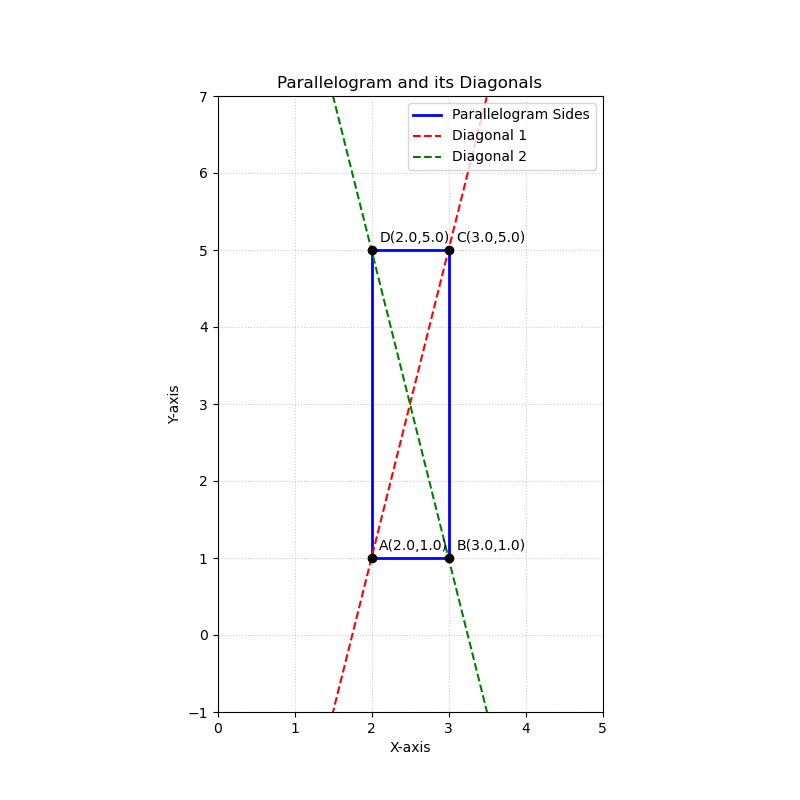
\includegraphics[width=\columnwidth, height=0.8\textheight, keepaspectratio]{figs/diagonals.png}     


\end{document}